
\section{Avoid  duplicately adding backup resource}
\label{sec:Avoid  duplicately adding backup resource}


Given one node fails, after applying Algorithm \ref{alg:DPAlg} to calculate the minimum additional resource, new physical node and physical path is added and involved to maintain the network function. If a physical node that does not hold any virtual node before physical node fail is added to be the backup node, we should set the physical node $s_j$ with $\xi(s_j)=1$ to indicate that this physical node is involved to hold virtual already.

As our survivable virtual network embedding problem wants to minimize the added backup resource when any one physical node fails instead of considering only one physical node failure, we should test each physical node fail one by one and add sufficient backup resource. As the backup resource only are used when node fails,  the  backup resource  should be shared when different physical node fails. If we directly apply cost defined in (\ref{eq:edge weight}) to calculate the backup resources when another physical node fails, as cost defined in (\ref{eq:edge weight}) does not consider the backup resource sharing, it will result in a problem of duplicately adding backup resource.

Considering the case of backup resource sharing,  we add the  $M(j)$ to the physical star structure to denote the set of virtual nodes migrated into  physical node $s_j$ in the case of physical node failure testing before.


\begin{equation}
PS(s_j)=(s_j, \phi^{-1}( s_j), c_j, F(j), \phi(N(\phi^{-1}( s_j))), \xi, M(j))
\end{equation}

As the backup resource should be added  only once, to facilitate expressing  this constraint, we define following equation.
\begin{equation}
\mu (x) = \left\{ {\begin{array}{*{20}{c}}
   x & {x > 0}  \\
   0 & {x \le 0}  \\
\end{array}} \right.
\end{equation}
When we test another physical node fails, instead of cost defined in (\ref{eq:edge weight}), we define a new cost function by taking consideration of the backup resource sharing when different node fails.
\begin{figure*}
  \centering
  % Requires \usepackage{graphicx}
    \begin{equation}
  \footnotesize
w(i,j) = \left\{ {\begin{array}{*{20}{c}}
   {C_s+{M_m}+\lambda {d_i}+\alpha \sum\limits_{v_k \in N(i)} {{d_{ik}}}}&{\xi(s_j)=0,v_i\notin \phi^{-1}(s_j)} \\
   {{M_m}+ \lambda \mu({d_i} - \mathop {\max }\limits_{{v_{i'}\in M(j)}} ( {{d_{i'}}} )) +\alpha\sum\limits_{v_k \in N(i)} {({d_{ik}} - \max\limits_{{v_{i'}\in M(j)}}({d_{i'k}}*{Pactive(\phi(v_k))}))}} & {\xi(s_j)=1,v_i\notin \phi^{-1}(s_j) }  \\
   { \alpha\sum\limits_{v_k \in N(i)} {\mu({d_{ik}} - \max\limits_{{v_{i'}\in M(j)}}({d_{i'k}}*{Pactive(\phi(v_k))}))}}  & {v_i\in \phi^{-1}(s_j)}  \\
\end{array}} \right.
    \label{eq:new edge weight}
    \end{equation}
\end{figure*}

As shown in (\ref{eq:new edge weight}), the resource cost is setting according to two cases.

Case 1: If virtual node $v_i$ is held by  physical node $s_j$ (i.e., ${{v_i} \in \left( {{\phi ^{ - 1}}({s_j}) \cup M(j)} \right)}$), when its neighbor $v_k \in N(i)$ fails (i.e., ${\phi \left( k \right) \notin \phi \left(N\left( {{\phi ^{ - 1}}({s_j})} \right)\right)}$), the path bandwidth cost is ${\sum\limits_{k \in N(i) \cap N(i')} {\mu({d_{ik}} - {d_{i'k}})}  + \sum\limits_{k \in \left( {N(i) - N(i')} \right)} {{d_{ik}}} }$ where ${v_{i'}}$ is the  virtual node that is migrated to physical node $s_j$ in pervious node failure testing (i.e., ${v_{i'}} \in M(j)$).
%$v_{i'_1},\ldots,v_{i'_{|M(j)|}}\in M(j)$
%${\sum\limits_{k \in ((N(i) \cap N(i'_1))\cup \ldots \cup(N(i) \cap N(i'_{M(j)})))} {\mu({d_{ik}} - {d_{i'k}})}  + \sum\limits_{k \in \left( {N(i) - N(i'_1)- \ldots - N(i'_{M(j)})} \right)} {{d_{ik}}} }$.

Case 2: Otherwise, if the virtual node $v_i$ is not held by the physical node (i.e., ${{v_i} \notin \left( {{\phi ^{ - 1}}({s_j}) \cup M(j)} \right)}$), besides the bandwidth cost ${\sum\limits_{k \in N(i) \cap N(i')} {\mu({d_{ik}} - {d_{i'k}})}  + \sum\limits_{k \in \left( {N(i) - N(i')} \right)} {{d_{ik}}} }$, VM migrate cost ${ {M_m}}$, $\delta$, and the capability cost ${\mu({d_i} - \mathop {\max }\limits_{{v_{i'}}} \left( {{d_{i'}}} \right))}$ should be counted for mapping the virtual star ($v_i$) to the physical node ($s_j$). If the backup capacity already allocated, ${\mathop {\max }\limits_{{v_{i'}}} \left( {{d_{i'}}} \right)}$ is larger than the amount needed  in current mapping (i.e., $d_i$), no additional resource is needed. Otherwise, the backup resource gap ${{d_i} - \mathop {\max }\limits_{{v_{i'}}} \left( {{d_{i'}}} \right)}$ is the further needed in current mapping, therefore, we use  ${\mu({d_i} - \mathop {\max }\limits_{{v_{i'}}} \left( {{d_{i'}}} \right))}$ to denote the capacity cost needed.



\begin{figure}
\centering
% Requires \usepackage{graphicx}
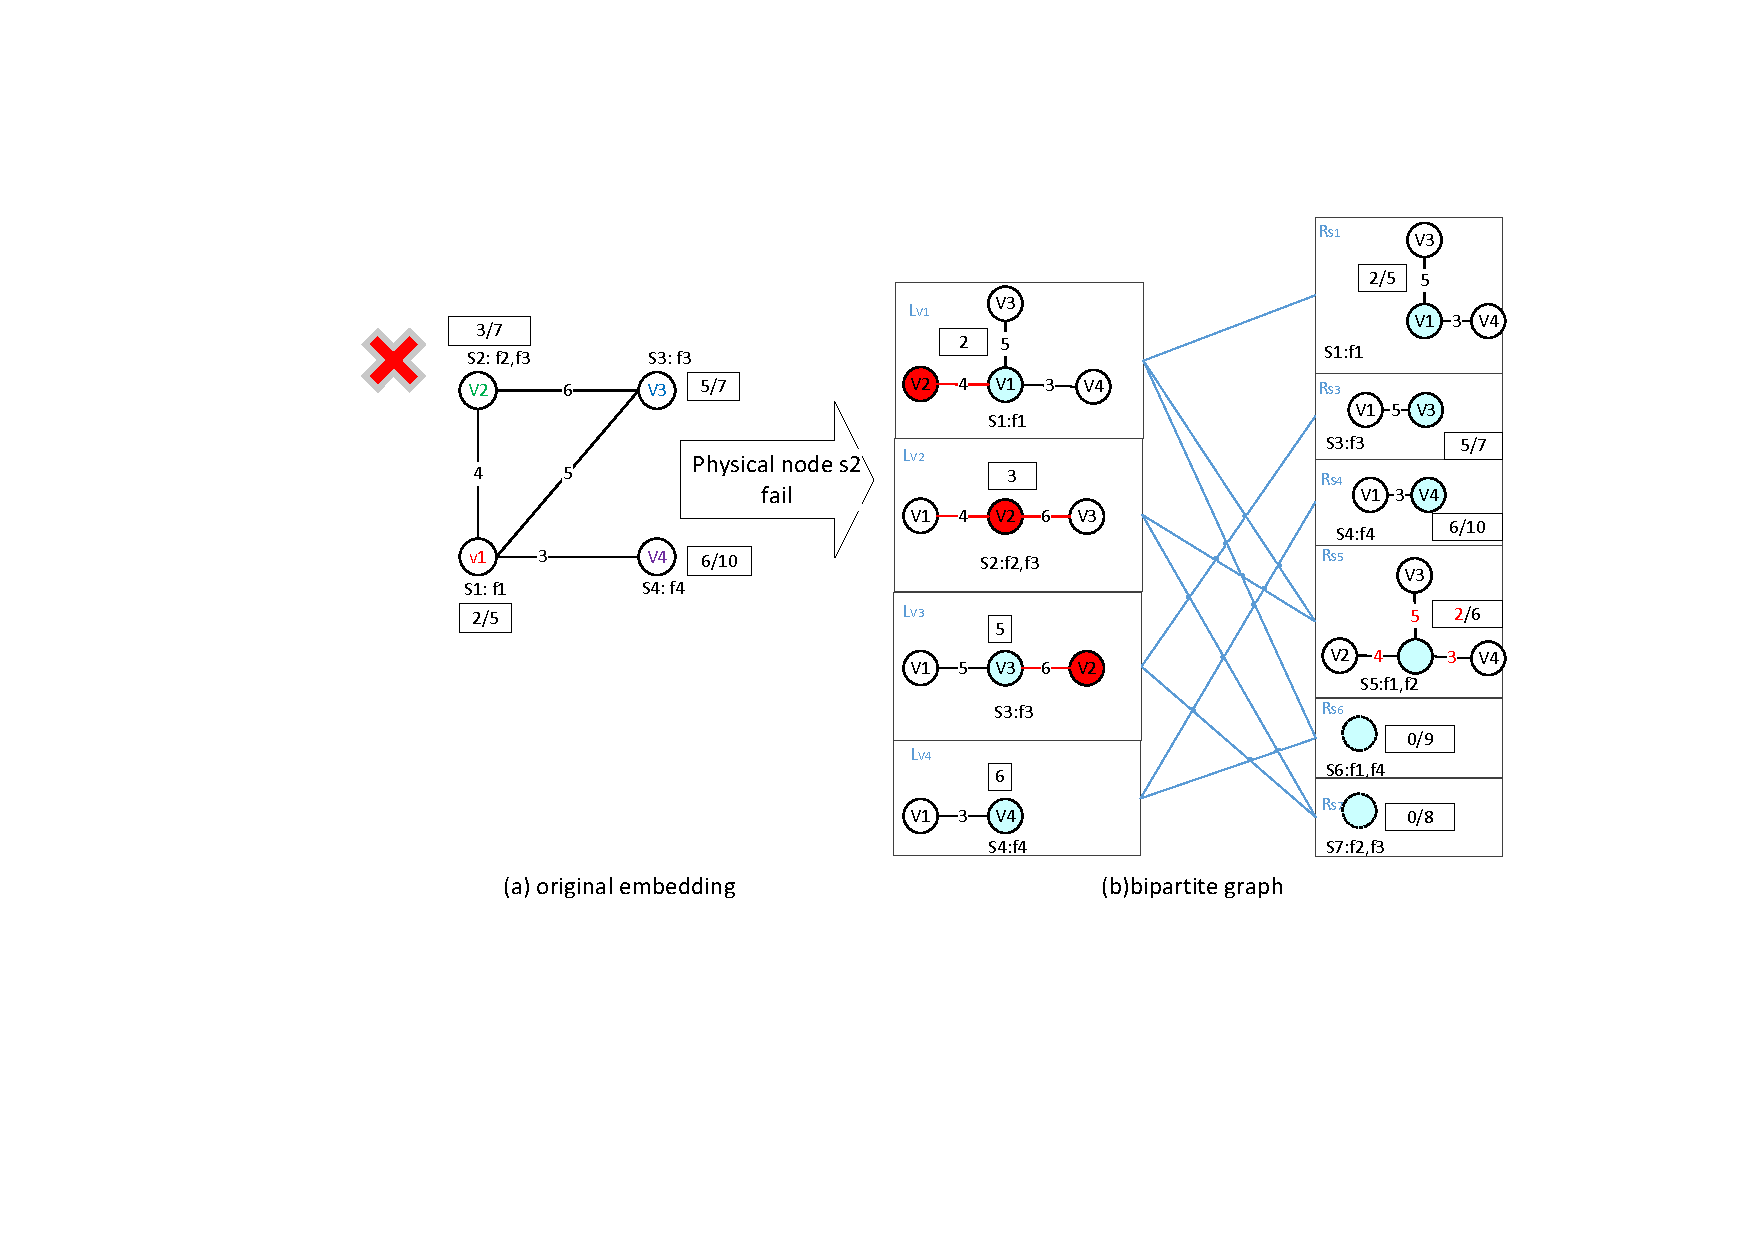
\includegraphics[width=3.5in]{Fig/StarRepresentationNode2}\\
  \caption{Components of VS($v_i$) and PS($s_j$) when we test physical node $s_2$  fails after we have tested physical node $s_1$ fails.}\label{fig:StarRepresentationNode2}
\end{figure}

%\[\begin{array}{*{20}{c}}
%{}&{PS(1)}&{PS(2)}&{PS(3)}&{PS(4)}&{PS(5)}&{PS(6)}&{PS(7)}\\
%{VS(1)}&{4\alpha }&\infty &\infty &\infty &{{M_m}{\rm{ + }}4\alpha }&{{C_s} + {M_m} + 2\lambda  + 12\alpha }&\infty \\
%{VS(2)}&\infty &\infty &\infty &\infty &{{M_m} + 1\lambda  + 5\alpha }&\infty &{{C_s} + {M_m} + 3\lambda  + 10\alpha }\\
%{VS(3)}&\infty &\infty &{5\alpha }&\infty &\infty &\infty &{{C_s} + {M_m} + 5\lambda  + 11\alpha }\\
%{VS(4)}&\infty &\infty &\infty &0&\infty &{{C_s} + {M_m} + 6\lambda  + 3\alpha }&\infty
%\end{array}\]

\begin{figure}
\centering
% Requires \usepackage{graphicx}
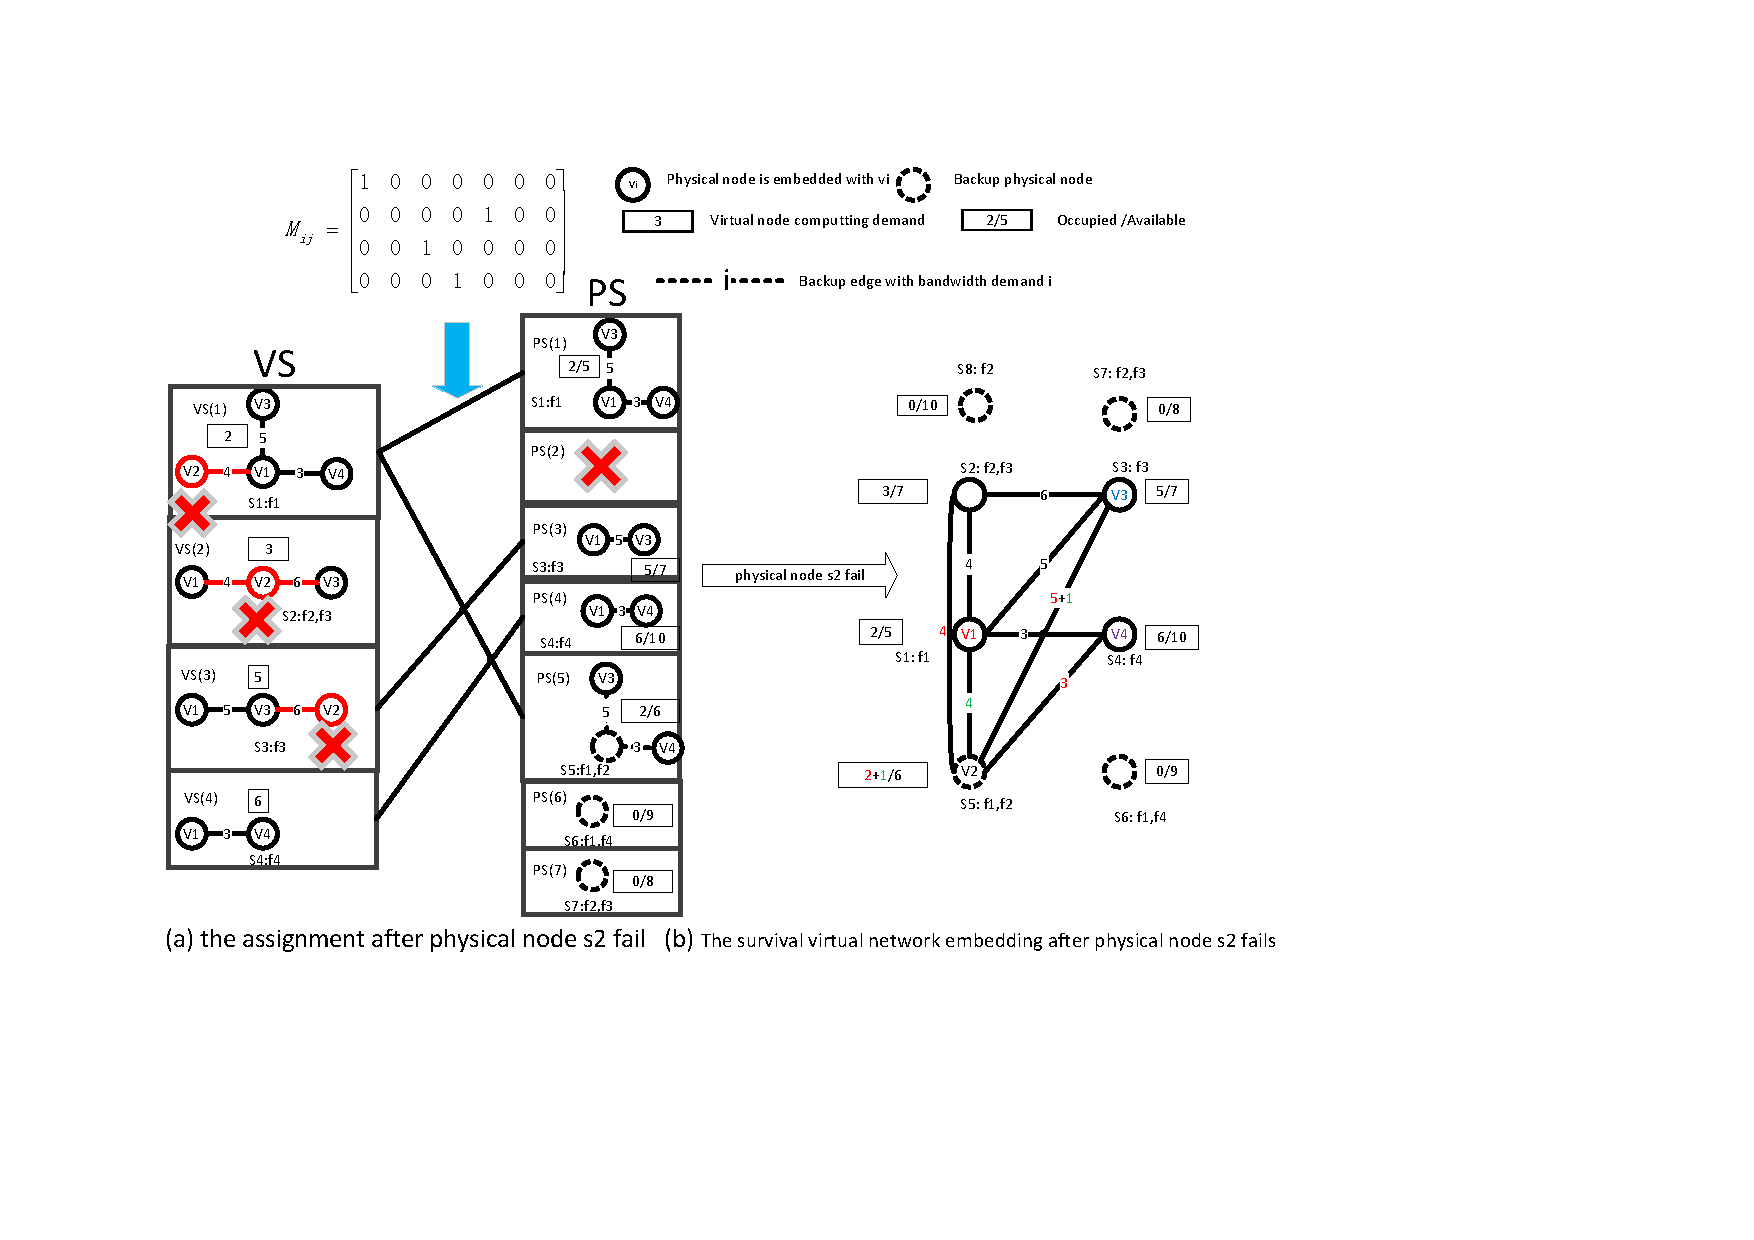
\includegraphics[width=4in]{Fig/Node2Failure}\\
  \caption{Node $s_2$ Failure}\label{fig:Node2Failure}
\end{figure}



Fig.\ref{fig:StarRepresentationNode2} uses an example to illustrate the the cost when we test physical node $s_2$ fails after we have tested physical node $s_1$ fails. From Fig.\ref{fig:Node1Failure}, we know when physical node $s_1$ fails, physical node $s_5$ is added as the backup node to hold virtual node $v_1$ instead of $s_1$. Therefore, in the  edge weight matrix, the cost of mapping $v_1$ to $s_5$ is  $e(1,5)=0$ as the backup resource of mapping $v_1$ to $s_5$ has been added when physical node $s_1$ fails. The cost of mapping $v_2$ to $s_5$ is , which including the additional capacity cost (), the bandwidth cost (), and the migration cost (). In the example, the capacity cost is $d_2-d_1=1$ instead of $d_2=3$. This is because that the amount of capacity $d_1=2$ is added as the backup capacity when $s_1$ fails, when $s_2$ fails, only $d_2-d_1=1$ is further needed to hold $v_2$.


.................................


For $VS(v_2)$, as $v_3$ is originally hold by $s_3$, however, when physical node $s_1$ fails, we could migrate virtual node $v_3$ onto physical node $s_2$, as $s_2$ is setup virtual machine before, therefore, cost include the virtual link bandwidth cost $11$, and node capacity cost 5, and virtual machine migration cost $M_m$.

Based method in Sec.\ref{lab:DynamicProgrammingEquation}, obtaining the optimal node mapping when physical node $s_1$ fails: $v_1 \rightarrow s_5$, $v_2 \rightarrow s_2$, $v_3 \rightarrow s_3$, $v_4 \rightarrow s_4$. The physical node $s_5$ begin setup and apply 2 node computing for virtual node $v_1$, and find three physical path corresponding virtual link $(v_1,v_2),(v_1,v_3),(v_1,v_4)$ with bandwidth constraints 4,5,3, respectively.

Fig.\ref{fig:StarRepresentationNode2} shows one example of such  bipartite graph with physical node $s_2$ fails after physical node $s_1$ failed. The edge weight of this   bipartite graph can be shown in  \ref{StarRepresentationNode2}(c).
As shown in Fig.\ref{fig:StarRepresentationNode2} , the optimal virtual node mapping matrix is $M_{ij}=\left[ {\begin{array}{*{20}{c}}
1&0&0&0&0&0&0\\
0&0&0&1&0&0&0\\
0&1&0&0&0&0&0\\
0&0&1&0&0&0&0
\end{array}} \right]$.

%$M_{ij}=\left[ {\begin{array}{*{20}{c}}
%0&0&0&0&1&0&0\\
%1&0&0&0&0&0&0\\
%0&1&0&0&0&0&0\\
%0&0&1&0&0&0&0
%\end{array}} \right]$.



For $VS(v_1)$, as $v_1$ is originally hold by $s_1$, however, when physical node $s_2$ fails, we could find a alternate physical node $s_5$ as migrated node for virtual node $v_1$, and the physical node $s_5$ own backup node computation and edge bandwidth resource because former physical node $s_1$ failure situation, so that when physical node $s_2$ fail the edge that connect $VS(v_1)$ and $PS(s_5)$ with the edge weight being $M_m$ .


For $VS(v_2)$, as $v_2$ is originally hold by $s_2$, however, when physical node $s_2$ fails, we could find a alternate physical node $s_5$ as migrated node for virtual node $v_2$, and the physical node $s_5$ own backup node computation and edge bandwidth resource because former physical node $s_1$ failure situation, so that when physical node $s_2$ fail the edge that connect $VS(v_1)$ and $PS(s_5)$ with the edge weight being $M_m+(1)+5$, the physical node $s_5$ just apply more 1 node computation resource for migrating virtual node $v_2$ for original backup node computation(2 node computation) resource of physical node $s_5$. There are a path between physical node $s_5$ and physical node $s_3$ mapping virtual node $v_3$, therefor, just apply 1 edge bandwidth to add the path physical node $s_5$ to physical node $s_3$ for satisfying the edge between virtual node $v_2$ and virtual node $v_3$, finally the cost of augmented path bandwidth is 1+4=5.

Based method in Sec.\ref{lab:DynamicProgrammingEquation}, obtaining the optimal node mapping when physical node $s_2$ fails with physical node $s_1$ had been failed: $v_1 \rightarrow s_1$, $v_2 \rightarrow s_5$, $v_3 \rightarrow s_3$, $v_4 \rightarrow s_4$. The physical node $s_5$ had been setup and remain 2 backup node computing because of physical node $s_1$ failure, therefore, just apply more 1 node computing for virtual node $v_2$, and find three physical path corresponding virtual link $(v_1,v_2),(v_1,v_3),(v_1,v_4)$ with bandwidth constraints 4,5,3, respectively.



\section{Extend to multiple physical nodes' failure}
\label{sec:Extend to multiple physical nodes' failure}



\begin{figure}
\centering
% Requires \usepackage{graphicx}
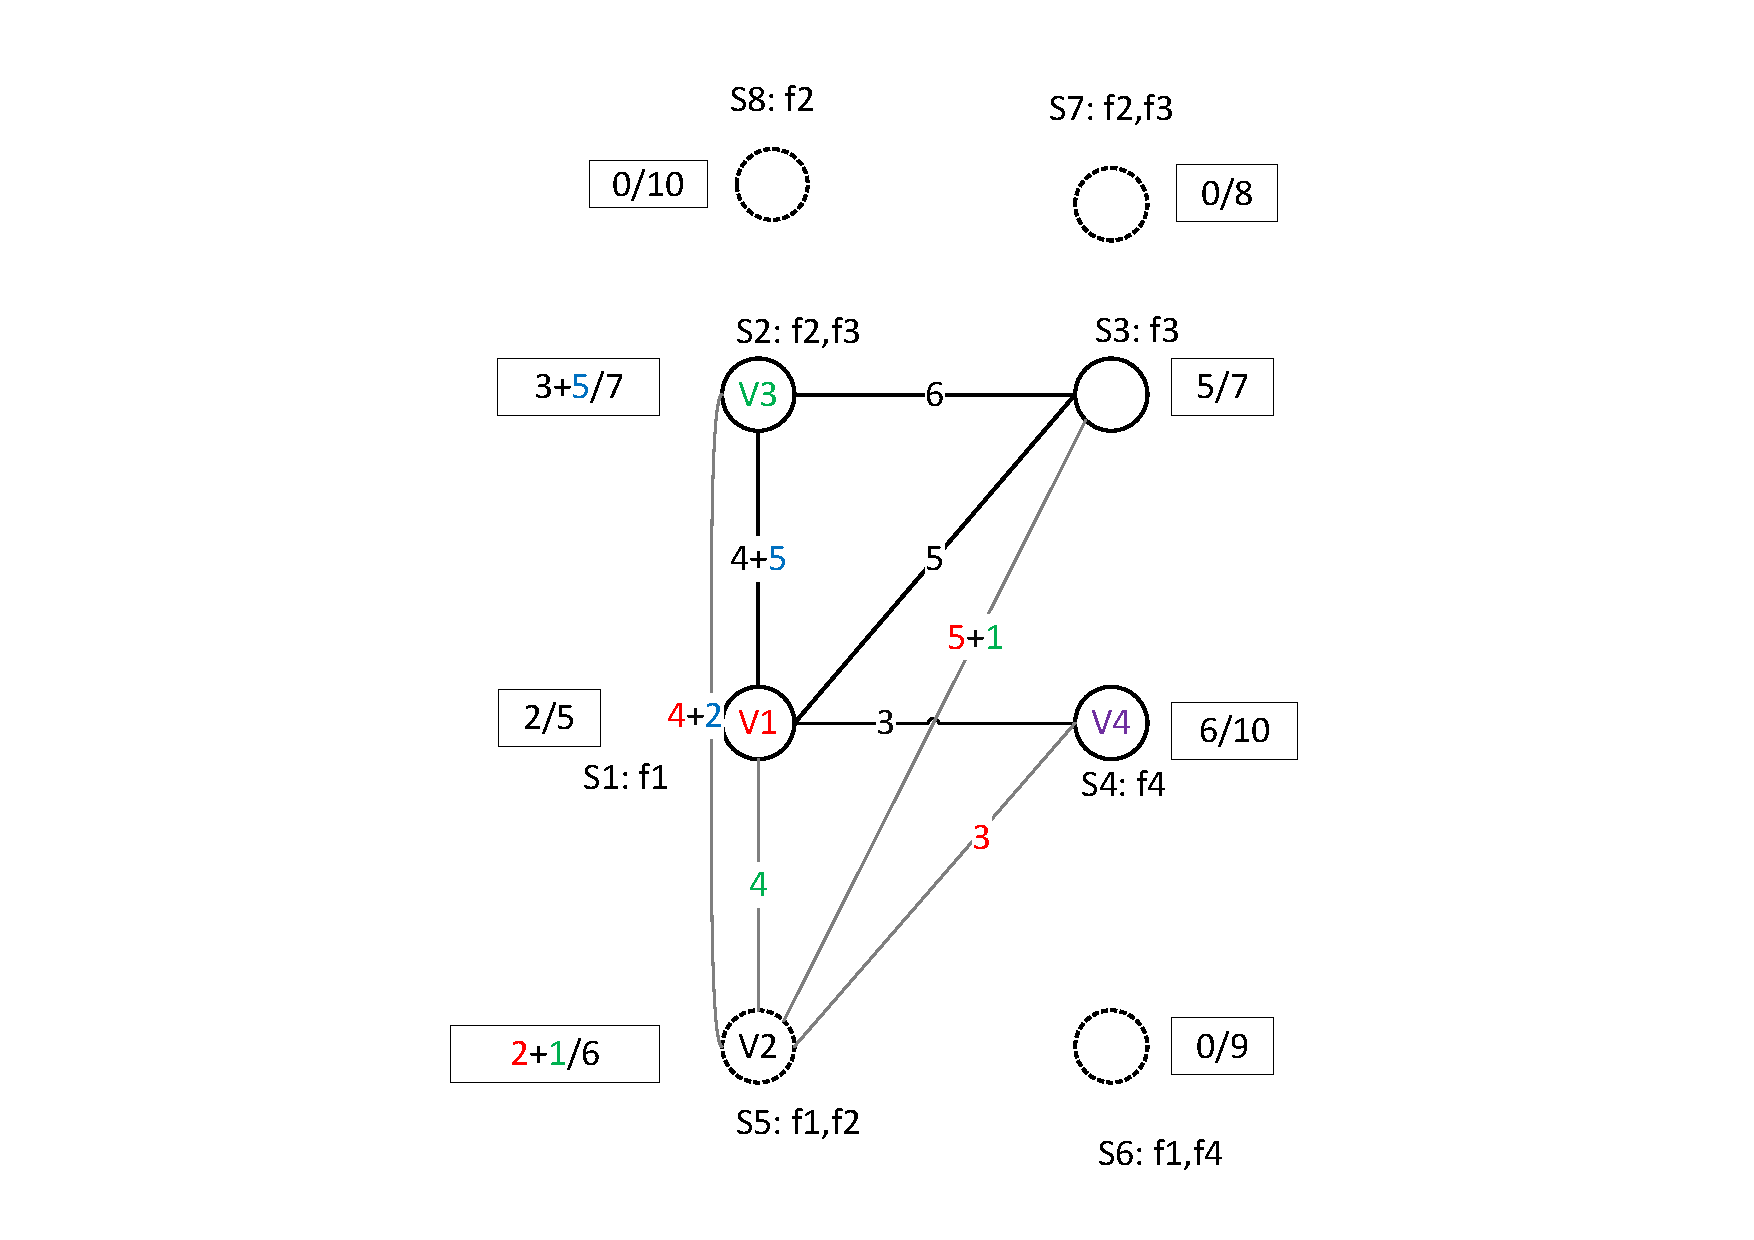
\includegraphics[width=2in]{Fig/Node3Failure}\\
  \caption{Node $s_3$ Failure}\label{fig:Node3Failure}
\end{figure}

\begin{figure}
\centering
% Requires \usepackage{graphicx}
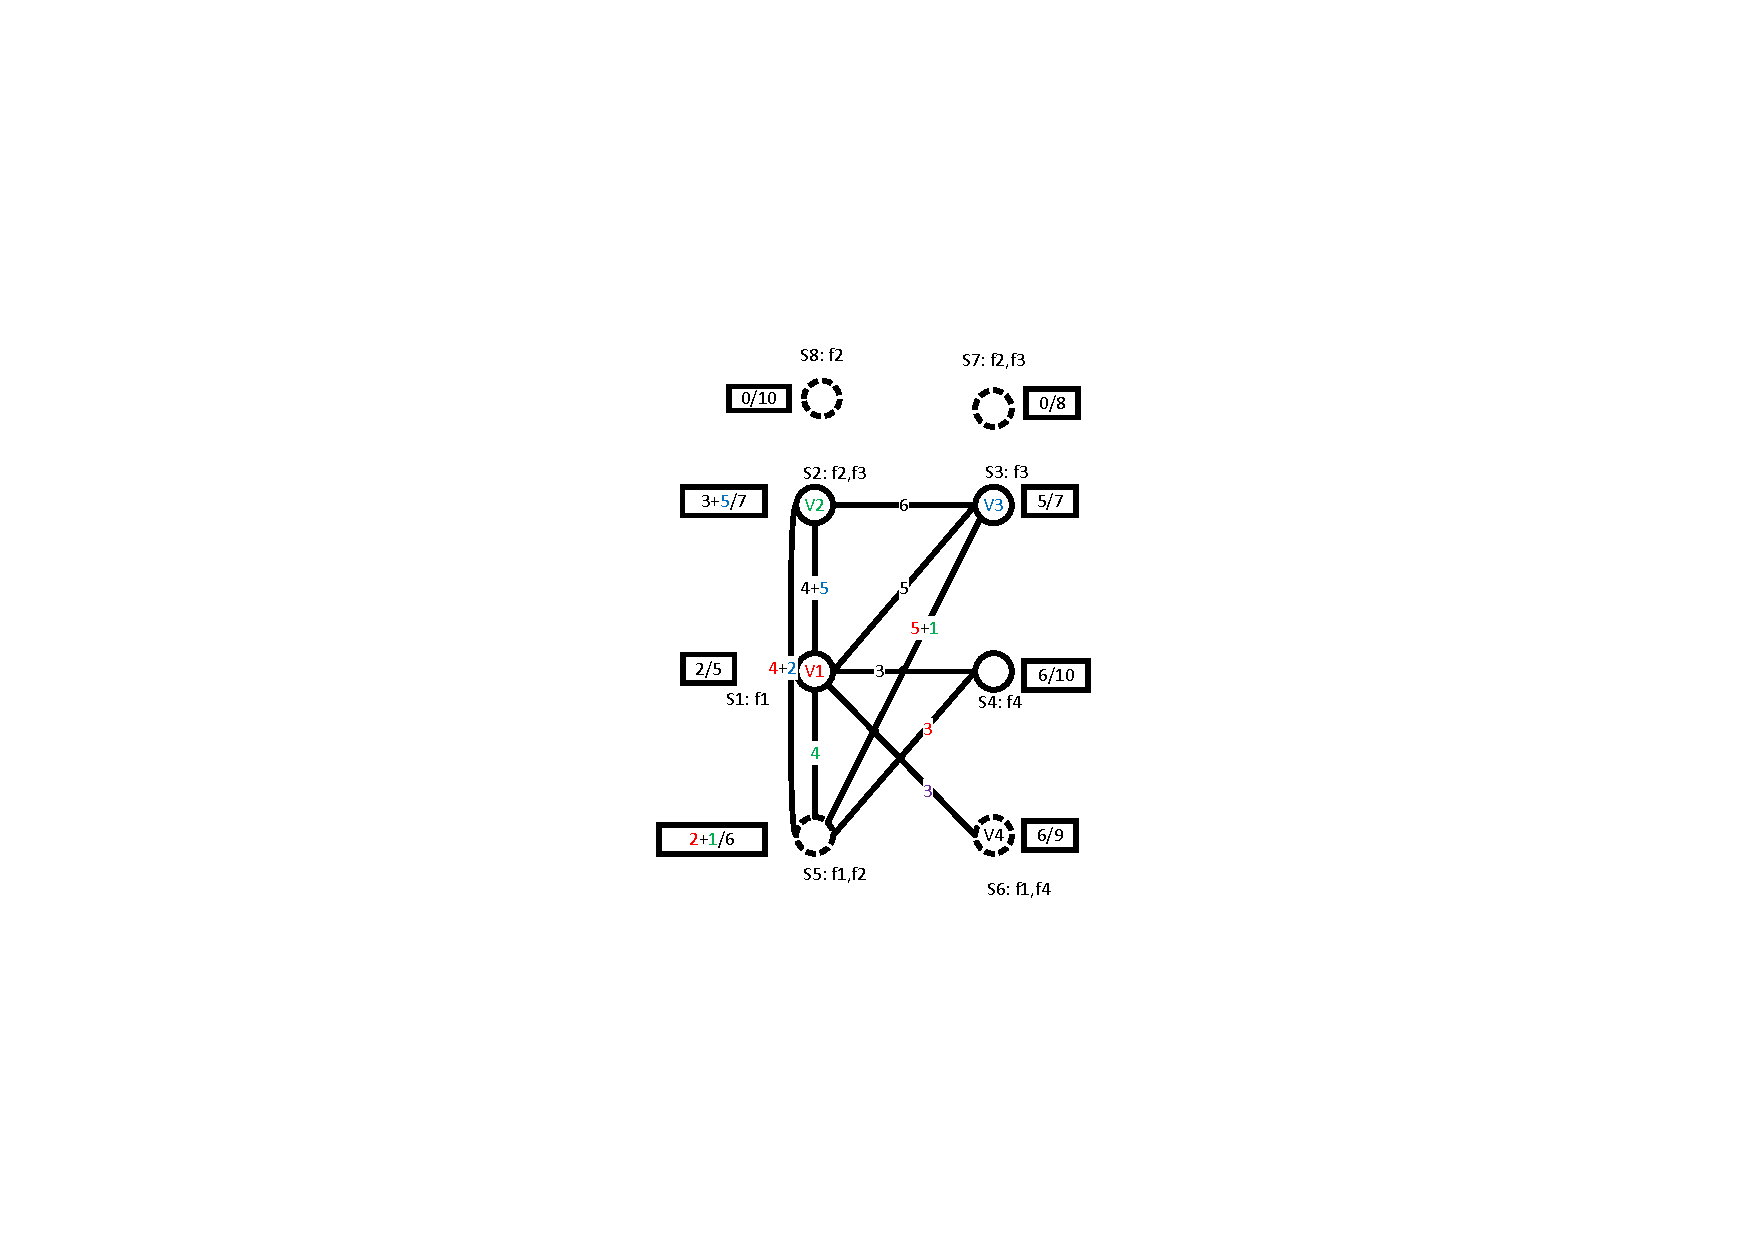
\includegraphics[width=2in]{Fig/Node4Failure}\\
  \caption{Node $s_4$ Failure}\label{fig:Node4Failure}
\end{figure}

Different from single node failure, we know that a large-scale regional failure could destroy one or more physical nodes to which some virtual nodes are mapped.
Although this paper focuses on providing the minimum  backup resource to provide
survivable service with single node failure, in this section, we show that with the well defined bipartite graph, we can easily  extend our solution to the scenario with multiple node failure.

Fig.\ref{fig:StarRepresentationTwoFailure} shows one example of such  bipartite graph when two physical nodes ($s_1$ and $s_2$) fail simultaneously. According to Eq.(\ref{eq:edge weight}), the edge weight of  this   bipartite graph can be shown in Fig. \ref{fig:StarRepresentationTwoFailure}(c). Obviously, with these edge weights setting, the survivable virtual network embedding problem under two node failure can be formulated using Eq.(\ref{eq:problem formulation}) and further be solved by our dynamic programming based algorithm.

\begin{figure}
\centering
% Requires \usepackage{graphicx}
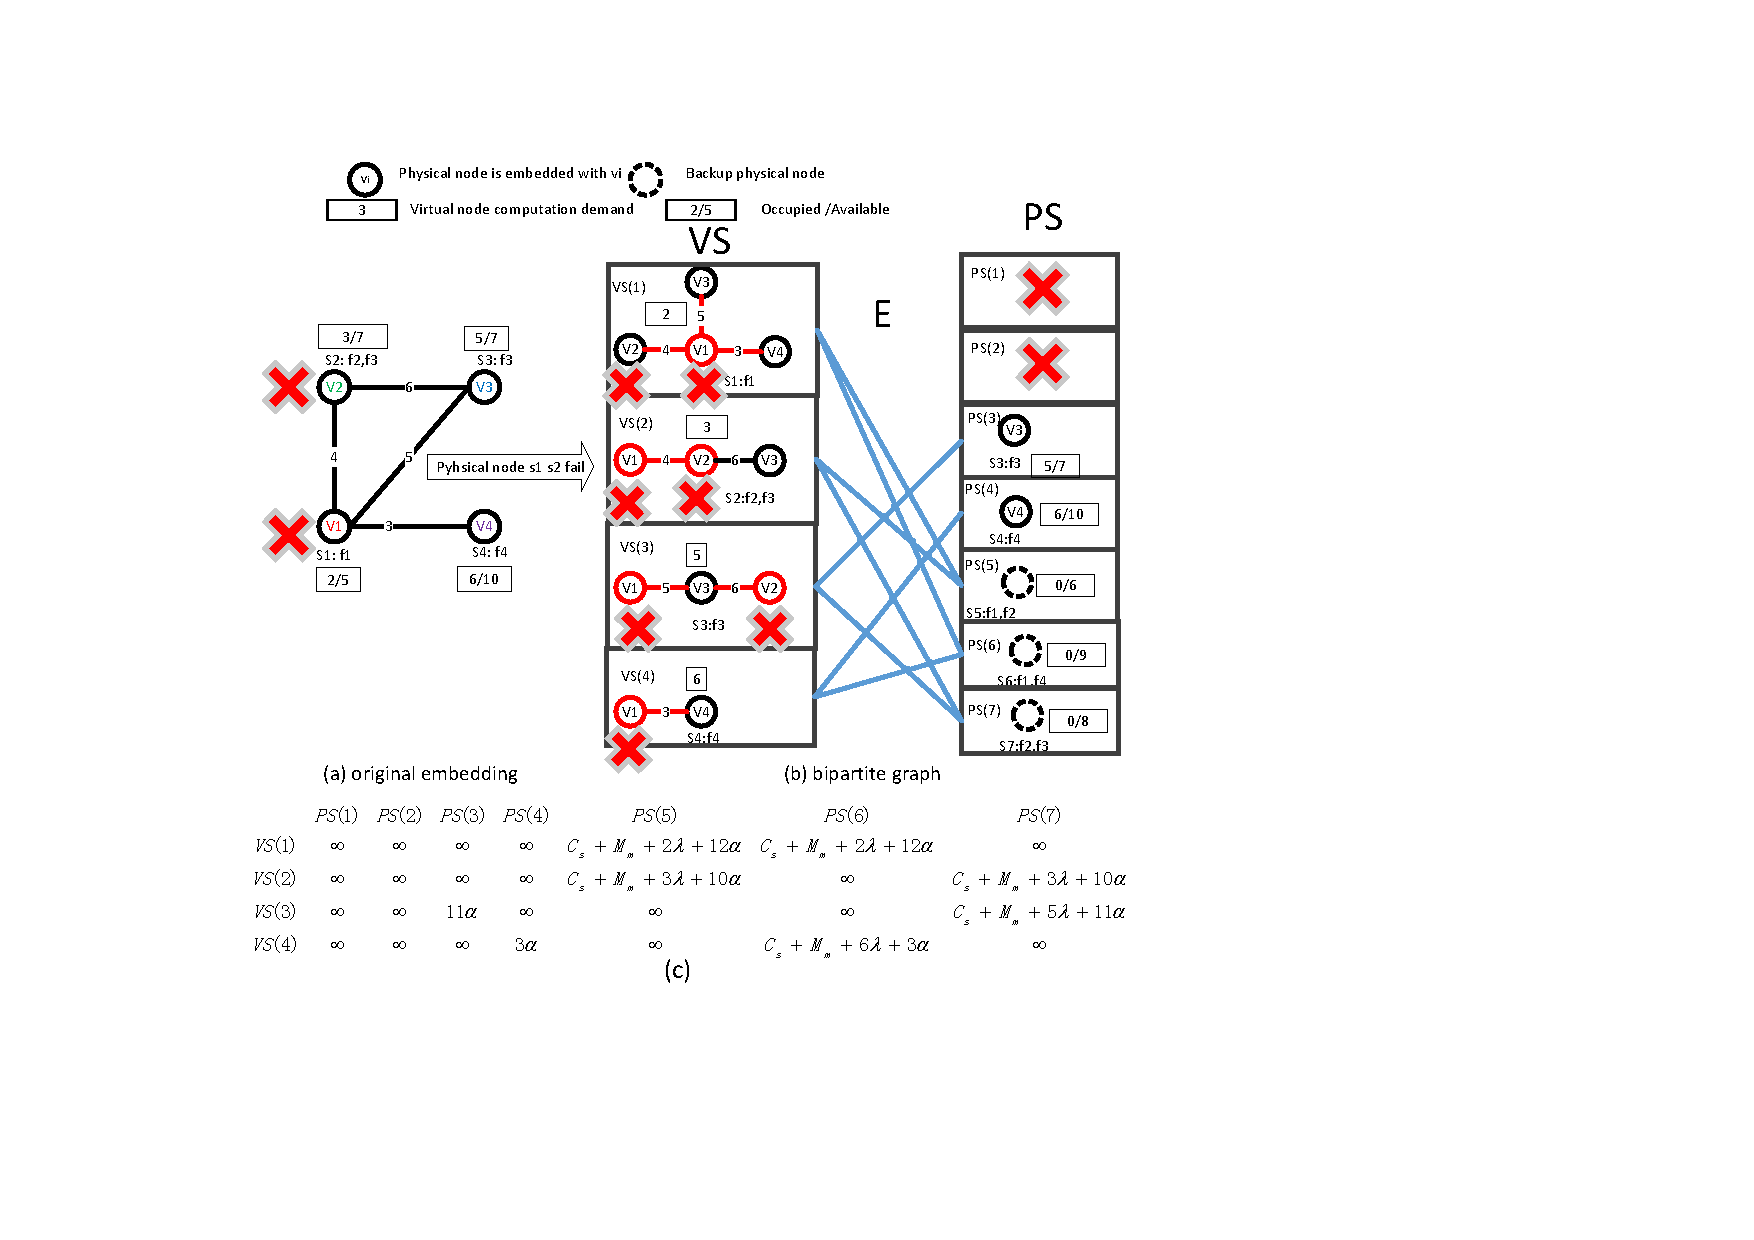
\includegraphics[width=3in]{Fig/StarRepresentationTwoFailure}\\
  \caption{Components of VS($v_i$) and PS($s_j$) when physical node $s_1$ and $s_2$ fail simultaneously}\label{fig:StarRepresentationTwoFailure}
\end{figure}


%\[\begin{array}{*{20}{c}}
%{}&{PS(1)}&{PS(2)}&{PS(3)}&{PS(4)}&{PS(5)}&{PS(6)}&{PS(7)}\\
%{VS(1)}&\infty &\infty &\infty &\infty &{{C_s} + {M_m} + 2\lambda  + 12\alpha }&{{C_s} + {M_m} + 2\lambda  + 12\alpha }&\infty \\
%{VS(2)}&\infty &\infty &\infty &\infty &{{C_s} + {M_m} + 3\lambda  + 10\alpha }&\infty &{{C_s} + {M_m} + 3\lambda  + 10\alpha }\\
%{VS(3)}&\infty &\infty &{11\alpha }&\infty &\infty &\infty &{{C_s} + {M_m} + 5\lambda  + 11\alpha }\\
%{VS(4)}&\infty &\infty &\infty &{3\alpha }&\infty &{{C_s} + {M_m} + 6\lambda  + 3\alpha }&\infty
%\end{array}\]

